\chapter{Replace with Third Chapter Name}\label{cha:c3_thirdchapter}

\begin{figure}
    \centering
    \begin{tikzpicture}
        \node[fill=yellow!80,ellipse] (origin) {Origin};
        \node[fill=blue!30,ellipse] (destination) at (15em,0) {Destination};
        \path (origin) edge[->] node[above,font=\footnotesize] {the journey}
        (destination);
    \end{tikzpicture}
    \caption{TikZ drawings will be output as SVG, which should be rendered by most modern browsers.}
\end{figure}

\begin{figure}
    \centering
    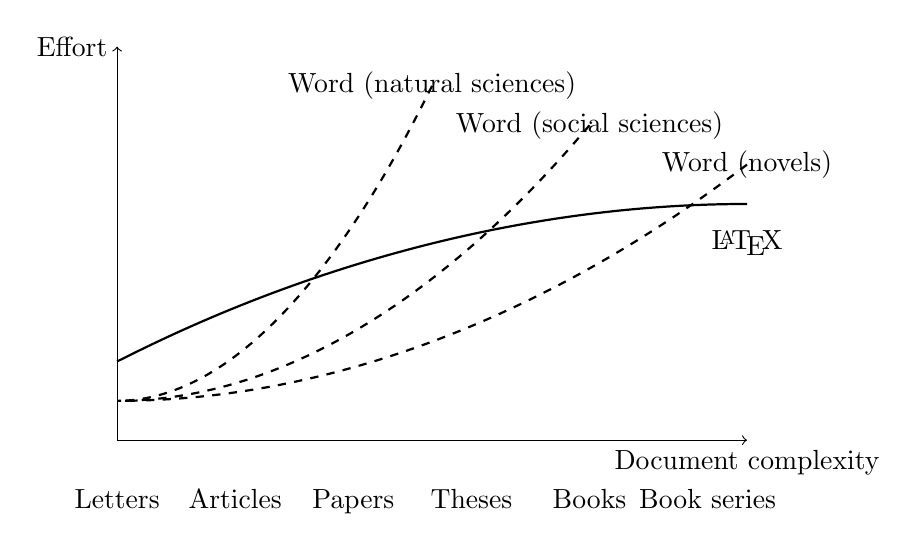
\begin{tikzpicture}

    % horizontal axis
    \draw[->] (0,0) -- (8,0) node[anchor=north] {Document complexity};
    \draw[->] (0,0) -- (0,5) node[anchor=east] {Effort};
    
    % labels
    \draw	(0,-0.5) node[anchor=north] {Letters}
    		(1.5,-0.5) node[anchor=north] {Articles}
    		(3,-0.5) node[anchor=north] {Papers}
    		(4.5,-0.5) node[anchor=north] {Theses}
    		(6,-0.5) node[anchor=north] {Books}
    		(7.5,-0.5) node[anchor=north] {Book series};
    
    \draw (8,3.5) node {Word (novels)};
    \draw (6,4) node {Word (social sciences)};
    \draw (4,4.5) node {Word (natural sciences)};
    \draw (8,2.5) node {\LaTeX{}};
    
    % Psis
    \draw[thick,dashed] (8,3.5) parabola[bend at end] (0,0.5);
    \draw[thick,dashed] (6,4) parabola[bend at end] (0,0.5);
    \draw[thick,dashed] (4,4.5) parabola[bend at end] (0,0.5);
    \draw[thick] (0,1) parabola[bend at end] (8,3);

\end{tikzpicture}
    \caption{Comparing complexity of \textit{Word} and \LaTeX{} depending on the application.}\label{fig:latexeffortcomplexity}
\end{figure}

\begin{figure}
    \centering
    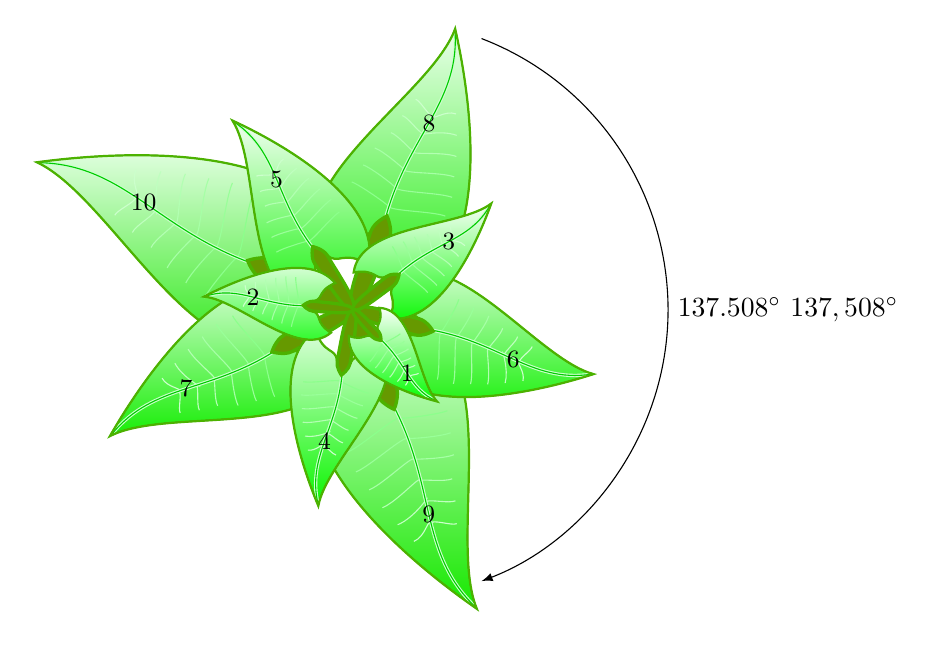
\begin{tikzpicture}
    \foreach \x in {10,...,1}
    {\draw[shade,bottom color=red!\x!green,top color=green!\x,x=0.3 pt,y=0.3 pt,scale={0.4+0.1*\x},rotate=222.5*\x] (0,0) .. 
    controls ( -11,  1) and ( -9, 50) .. (-10,80) ..
    controls ( -16, 60) and (-32, 75) .. (-50,40) .. 
    controls (-110,100) and (-0,230) ..  (  0,300)  node[below] (\x) {} ..
    controls (  45,230) and (110,100) .. ( 50,40) ..
    controls (  32, 75) and ( 16, 60) ..  ( 10,80) ..
    controls (   9, 50) and ( 11,  1) .. (  0,0) 
    -- cycle ;
    
    \draw[thin,green!45,x=0.3 pt,y=0.3 pt,scale={0.4+0.1*\x},rotate=222.5*\x] (-45,120) .. controls (-35,120) and (0,110) .. (-3,110) .. controls (0,105) and (40,120) .. (55,120);
    \draw[thin,green!40,x=0.3 pt,y=0.3 pt,scale={0.4+0.1*\x},rotate=222.5*\x] (-40,140) .. controls (-30,140) and (0,130) .. (-3,130) .. controls (0,125) and (40,140) .. (55,140);
    \draw[thin,green!35,x=0.3 pt,y=0.3 pt,scale={0.4+0.1*\x},rotate=222.5*\x] (-35,160) .. controls (-25,160) and (0,150) .. (0,150) .. controls (0,145) and (35,160) .. (50,160);
    \draw[thin,green!30,x=0.3 pt,y=0.3 pt,scale={0.4+0.1*\x},rotate=222.5*\x] (-25,180) .. controls (-17,180) and (0,170) .. (3,170) .. controls (0,165) and (30,180) .. (45,180);
    \draw[thin,green!25,x=0.3 pt,y=0.3 pt,scale={0.4+0.1*\x},rotate=222.5*\x] (-20,200) .. controls (-13,200) and (0,190) .. (6,190) .. controls (0,185) and (20,200) .. (38,200);
    \draw[thin,green!20,x=0.3 pt,y=0.3 pt,scale={0.4+0.1*\x},rotate=222.5*\x] (-13,220) .. controls (-8,220) and (3,210) .. (8,210) .. controls (10,205) and (18,220) .. (30,220);
    \draw[very thick,green!20,x=0.3 pt,y=0.3 pt,scale={0.4+0.1*\x},rotate=222.5*\x] (0,90) .. controls (-10,180) and (30,230) .. (1,297);
    \draw[thin,black!20!green,x=0.3 pt,y=0.3 pt,scale={0.4+0.1*\x},rotate=222.5*\x] (0,90)  .. controls (-10,180) and (30,230)  .. (1,297) node[midway,black] (num\x) {\small\x};
    \draw[very thick,red!30!green,fill=red!40!green,x=0.3 pt,y=0.3 pt,scale={0.4+0.1*\x},rotate=222.5*\x] 
    (0,0) .. 
    controls ( -11,  1) and ( -9, 50) ..
    (-10,80) .. 
    controls (-10,90) and (0,100) .. (0,100) ..
    controls (0,100) and (10,90) .. (10,80)..
    controls (   9, 50) and ( 11,  1) .. (  0,0) 
    -- cycle;
    \draw[thick,red!30!green,x=0.3 pt,y=0.3 pt,scale={0.4+0.1*\x},rotate=222.5*\x] (0,0) .. 
    controls ( -11,  1) and ( -9, 50) .. (-10,80) ..
    controls ( -16, 60) and (-32, 75) .. (-50,40) .. 
    controls (-110,100) and (-0,230) ..  (  0,300) ..
    controls (  45,230) and (110,100) .. ( 50,40) ..
    controls (  32, 75) and ( 16, 60) ..  ( 10,80) ..
    controls (   9, 50) and ( 11,  1) .. (  0,0) 
    -- cycle ;
    }
    \draw[->,>=latex,x=0.3 pt,y=0.3 pt,black] ([xshift=6pt] 8.east) arc (69:-69:350) node[midway,right] {$137.508^\circ$ $137,508^\circ$};
\end{tikzpicture}

    \caption{Example of a drawing made in TikZ.}\label{fig:leaves-golden-cut}
\end{figure}

\begin{figure}
    \centering
    \begin{tikzpicture}
    % Define styles of various tikz elements.
    \tikzstyle{textbox} = [rounded corners, text width=60pt, minimum height=50pt,text centered,draw=black]
    \tikzstyle{arrow} = [thick,->,>=latex]
    \tikzstyle{block} = [rectangle,textbox]
    \tikzstyle{textarr} = [rectangle,align=center,fill=white]

    \node (latex) [block] {\LaTeX{}\\document};
    \node (overleaf) [block, left=of latex] {Overleaf};
    \node (pdf) [block, above left=of overleaf] {PDF}; % xelatex
    \node (html) [block, above right=of overleaf] {HTML}; % pdfLaTeX + tex4ht
    
    \node (print) [block, above= of pdf] {Printed\\book};
    \node (mobi) [block, above left=of html] {MOBI\\(Amazon)}; % Kindle Previewer
    \node (epub) [block, above= of html] {EPUB\\(GooglePlay)}; % Calibri
    
    \draw[out=90,in=270] [arrow] (overleaf) to node[textarr] {XeLaTeX} (pdf);
    \draw[out=90,in=270] [arrow] (overleaf) to node[textarr] {pdfLaTeX\\tex4ht} (html);
    
    \draw [arrow] (latex) -- (overleaf);
    \draw [arrow] (pdf) -- (print);
    
    \draw[out=90,in=270] [arrow] (html) to node[textarr] {Kindle\\Previewer} (mobi);
    \draw [arrow] (html) -- node[textarr] {Calibri} (epub);
\end{tikzpicture}
    \caption{Example 2 of a drawing made in TikZ.}\label{fig:buildchain}
\end{figure}